\documentclass[12pt]{article}

\usepackage{palatino}
%\usepackage{times}
\usepackage{graphicx}
\usepackage{wasysym} % for check symbol
\usepackage{color}

% revise the page layout
\setlength{\hoffset}{-0.35in}
\setlength{\voffset}{-0.40in}
\setlength{\topmargin}{-0.7in}
\setlength{\oddsidemargin}{-0.55in}
\setlength{\evensidemargin}{-0.55in}
\setlength{\textwidth}{7.8in}
\setlength{\headheight}{0in}
\setlength{\headsep}{0in}
\setlength{\footskip}{0in}
\setlength{\textheight}{4in}

\setlength{\parskip}{6pt}
\setlength{\parindent}{0pt}

\definecolor{myred}{rgb}{1,0,0}
\definecolor{mygreen}{rgb}{0,0.8039216,0}
\definecolor{myblue}{rgb}{0,0,1}
\definecolor{myorange}{rgb}{0.9333333,0.6039216,0}
%\definecolor{myred}{rgb}{0,0,0}
%\definecolor{mygreen}{rgb}{0,0,0}
%\definecolor{myblue}{rgb}{0,0,0}
%\definecolor{myorange}{rgb}{0,0,0}

\pdfpageheight2.1in
\pdfpagewidth7.95in


\pagestyle{empty}

\begin{document}

\sffamily

\begin{minipage}[t]{2.05in}
\vspace*{0cm}

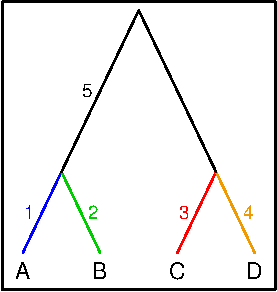
\includegraphics{phylotree.pdf}

\end{minipage} \hfill
\begin{minipage}[t]{5.65in}
\vspace*{0cm}

\renewcommand{\arraystretch}{1.2}
\hfill 
\begin{tabular}{cccccc}
\hline 
& \multicolumn{5}{c}{QTL position (partition of taxa)} \\ \cline{2-6}
Cross        & {\color{myblue} 1 (A$|$BCD)} & {\color{mygreen} 2 (B$|$ACD)} & {\color{myred} 3 (C$|$ABD)} & {\color{myorange} 4 (D$|$ABC)} & 5 (AB$|$CD) \\ \hline
A $\times$ B & $\checked$  & $\checked$  & $\times$    & $\times$    & $\times$ \\
A $\times$ C & $\checked$  & $\times$    & $\checked$  & $\times$    & $\checked$ \\ 
A $\times$ D & $\checked$  & $\times$    & $\times$    & $\checked$  & $\checked$ \\ 
B $\times$ C & $\times$    & $\checked$  & $\checked$  & $\times$    & $\checked$ \\ 
B $\times$ D & $\times$    & $\checked$  & $\times$    & $\checked$  & $\checked$ \\ 
C $\times$ D & $\times$    & $\times$    & $\checked$  & $\checked$  & $\times$ \\ 
\hline
\end{tabular}
\renewcommand{\arraystretch}{1.0}
\end{minipage}

\end{document}
